\documentclass[a4paper]{article}

%% Language and font encodings
\usepackage[english]{babel}
\usepackage[utf8x]{inputenc}
\usepackage[T1]{fontenc}

%% Sets page size and margins
\usepackage[a4paper,top=3cm,bottom=3cm,left=3cm,right=3cm,marginparwidth=1.75cm]{geometry}

%% Useful packages
\usepackage{amsmath}
\usepackage{graphicx}
\usepackage{url}
\usepackage[colorlinks=true, allcolors=blue]{hyperref}
\usepackage{amsfonts}
\usepackage{amsmath}
\usepackage{physics}
\usepackage{amssymb}
\usepackage{mathtools}

\numberwithin{equation}{subsection}
\newcommand{\mb}[1]{\mathbf{#1}}
\title{Magnetic propeties of a two dimentional electron gas strongly coupled to lights}
\author{K.Dini, O.V. Kibis and I.A. Shelykh}
\numberwithin{equation}{section}

\begin{document}

\maketitle

\section{Schrödinger problem for Landau levels in dressed 2DEG}

Our analysis is consider on 2 dimentional electronic gas which has distrubuted in $(x,y)$ plane in configuration space. We are going to examine the properties of 2DEG with stationary magnetic field
\begin{equation} \label{1.1}
  \vb{B} = (0,0,B)^T
\end{equation}
which directed on $z$ axis and a linearly $y$-polarized strong electomagnetic wave (dressing field) with electric field given by
\begin{equation} \label{1.2}
  \vb{E} = (0,E\sin(\omega t),0)^T
\end{equation}
which also propagate in $z$ direction. Here $B$ and $E$ represent the amplitude of the stationary magnetic field and electric field of dressing field.
\begin{figure}[ht!]
  \centering
  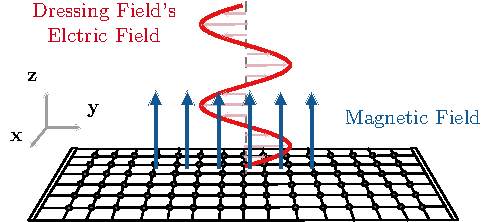
\includegraphics[scale=0.9]{figures/fig1.pdf}
  \caption{Stationary magnetic filed (blue color) and Strong EM wave (red color) applied to the 2DEG.}
  \label{fig:1.1}
\end{figure}

\noindent
Using Landau gauge for the stationary magnetic field we can represent it using vector potential as
\begin{equation} \label{1.3}
  \vb{A}_{s} = (-By,0,0)^T
\end{equation}
and choosing Coulomb gauge the dressing field can be present as the following vector potential
\begin{equation} \label{1.4}
  \vb{A}_{d}(t) = (0,[E/\omega ]\cos(\omega t),0)^T.
\end{equation}
Now the Hamiltonian of an electron in 2DEG can be reads as
\begin{equation} \label{1.5}
  \hat{H}_e(t) = \frac{1}{2m_e}\Big[\hat{\vb{p}} - e\big(\vb{A}_{s}+\vb{A}_{d}(t)\big)\Big]^2
\end{equation}
where $m_e$ is the effective mass of the electron and $e$ is the magnitude (without considering the sign of the charge) of the electron charge. This can be simplified to
\begin{equation} \label{1.6}
  \hat{H}_e(t) = \frac{1}{2m_e}\Big[
    (\hat{p}_x + eBy)\vb{e}_x +
    (\hat{p}_y - \frac{eE}{\omega}\cos(\omega t))\vb{e}_y
  \Big]^2
\end{equation}
where $\vb{e}_x$ and $\vb{e}_y$ are unit vectors along $x$ and $y$ directions respectively. Moreover,
\begin{equation} \label{1.7}
  \hat{H}_e(t) = \frac{1}{2m_e}\Big[
    (\hat{p}_x + eBy)^2 +
    (\hat{p}_y - \frac{eE}{\omega}\cos(\omega t))^2
  \Big]
\end{equation}
Since $[\hat{H}_e(t),\hat{p}_x] =0$ both operators share same eigenvalue and eigen functions which are free electron wave functions. Therefore we can modify the Hamiltonian as follows
\begin{equation} \label{1.8}
  \hat{H}_e(t) = \frac{1}{2m_e}\Big[
    ({p}_x + eBy)^2 +
    (\hat{p}_y - \frac{eE}{\omega}\cos(\omega t))^2
  \Big].
\end{equation}
Using momentum operator definition
\begin{equation} \label{1.9}
  \hat{p}_y = -i\hbar \pdv{y}
\end{equation}
we can modify Eq. \eqref{1.8} as
\begin{equation} \label{1.10}
  \begin{aligned}
    \hat{H}_e(t) & = \frac{1}{2m_e}\Big[
      ({p}_x + eBy)^2 +
      \Big(-i\hbar \pdv{y}- \frac{eE}{\omega}\cos(\omega t)\Big)^2
    \Big] \\
    & = \frac{1}{2m_e}\Big[
      ({p}_x + eBy)^2 +
      \Big(i\hbar \pdv{y} + \frac{eE}{\omega}\cos(\omega t)\Big)^2
    \Big].
  \end{aligned}
\end{equation}
Define the \textit{center of the cyclotron orbit} along $y$ axis as
\begin{equation} \label{1.11}
  y_0 \equiv \frac{-p_x}{eB}
\end{equation}
and the \textit{cyclotron frequency} as
\begin{equation} \label{1.12}
  \omega_0 \equiv \frac{eB}{m_e}.
\end{equation}
Then the Hamiltonian will leads to
\begin{equation} \label{1.13}
    \hat{H}_e(t) =
      \frac{m_e \omega_0^2}{2}(y-y_0)^2 +
      \frac{1}{2m_e}\Big(i\hbar \pdv{y}+\frac{eE}{\omega}\cos(\omega t)\Big)^2
\end{equation}
\begin{equation} \label{1.14}
  \begin{aligned}
    \hat{H}_e(t) =
      \frac{m_e \omega_0^2}{2}(y-y_0)^2 +
      \frac{1}{2m_e}\Big(
      -\hbar^2 \pdv[2]{y} & +
      i\hbar \pdv{y}\bigg[\frac{eE}{\omega}\cos(\omega t) \bigg] \\ & +
      \frac{i\hbar eE}{\omega}\cos(\omega t) \pdv{y}+
      \frac{e^2E^2}{\omega^2}\cos[2](\omega t)
      \Big)
  \end{aligned}
\end{equation}
\begin{equation} \label{1.15}
  \begin{aligned}
    \hat{H}_e(t) =
      \frac{m_e \omega_0^2}{2}(y-y_0)^2 +
      \frac{1}{2m_e}\Big(
      -\hbar^2 \pdv[2]{y} +
      \frac{2i\hbar eE}{\omega}\cos(\omega t) \pdv{y}+
      \frac{e^2E^2}{\omega^2}\cos[2](\omega t)
      \Big).
  \end{aligned}
\end{equation}
Let
\begin{equation} \label{1.16}
    (y - y_0) \rightarrow y
\end{equation}
and then this becomes
\begin{equation} \label{1.17}
  \begin{aligned}
    \hat{H}_e(t) =
      \frac{m_e \omega_0^2}{2}y^2 +
      \frac{1}{2m_e}\Big(
      -\hbar^2 \pdv[2]{y} +
      \frac{2i\hbar eE}{\omega}\cos(\omega t) \pdv{y}+
      \frac{e^2E^2}{\omega^2}\cos[2](\omega t)
      \Big).
  \end{aligned}
\end{equation}
Now assume that the solution for the time-dependent schrödinger equation
\begin{equation} \label{1.18}
    i \hbar \dv{\psi}{t} = \hat{H}_e(t)\psi
\end{equation}
can be represent by the following form
\begin{equation} \label{1.19}
    \psi(\vb{r},t) = \frac{1}{\sqrt{L_x}} \exp\bigg(
      \frac{ip_x x}{\hbar} +
      \frac{ieE(y-y_0)}{\hbar \omega}\cos(\omega t)
    \bigg) \phi(y-y_0,t).
\end{equation}
Using the same subtution from Eq. \eqref{1.16} this becomes
\begin{equation} \label{1.20}
    \psi(x,y,t) = \frac{1}{\sqrt{L_x}} \exp\bigg(
      \frac{ip_x x}{\hbar} +
      \frac{ieEy}{\hbar \omega}\cos(\omega t)
    \bigg) \phi(y,t).
\end{equation}
Defining
\begin{equation} \label{1.21}
    \varphi(x,y,t) \equiv \frac{1}{\sqrt{L_x}} \exp\bigg(
      \frac{ip_x x}{\hbar} +
      \frac{ieEy}{\hbar \omega}\cos(\omega t)
    \bigg)
\end{equation}
we can simply the the Eq. \eqref{1.20} as
\begin{equation} \label{1.22}
    \psi(x,y,t) = \varphi(x,y,t) \phi(y,t).
\end{equation}
Let's subtitue Eq. \eqref{1.20} and Eq. \eqref{1.17} into Eq. \eqref{1.18} and we can observe that
\begin{equation} \label{1.23}
  \begin{aligned}
    \text{L.H.S} & = i \hbar \dv{\psi}{t} =
    i \hbar \bigg( \dv{\varphi}{t} \phi + \dv{\phi}{t} \varphi \bigg) =
    i \hbar \bigg(
      \Big[\frac{-ieEy}{\hbar}\sin(\omega t)\Big]\varphi\phi +
      \varphi  \dv{\phi}{t}
    \bigg) \\
    & =
    \big[{eEy}\sin(\omega t)\big]\varphi\phi +
    i \hbar\varphi  \dv{\phi}{t}
  \end{aligned}
\end{equation}
and
\begin{equation} \label{1.24}
  \begin{aligned}
    \text{R.H.S} & = \hat{H}_e(t)\psi \\
    & =
    \bigg[
    \frac{m_e \omega_0^2}{2}y^2 +
    \frac{1}{2m_e}\Big(
    -\hbar^2 \pdv[2]{y} +
    \frac{2i\hbar eE}{\omega}\cos(\omega t) \pdv{y}+
    \frac{e^2E^2}{\omega^2}\cos[2](\omega t)
    \Big) \bigg]
    \varphi\phi
  \end{aligned}
\end{equation}
where we will can calculate this part by part as follows:
\begin{equation} \label{1.25}
  \begin{aligned}
    \frac{-\hbar^2}{2m_e}\pdv[2]{y}(\varphi\phi) & =
    \frac{-\hbar^2}{2m_e} \pdv{y}\bigg[
      \Big(\frac{ieE}{\hbar \omega} \cos(\omega)t\Big)\varphi\phi +
      \varphi\pdv{\phi}{y}
    \bigg] \\
    & =
    \frac{-\hbar^2}{2m_e} \bigg[
      \Big(\frac{ieE}{\hbar \omega} \cos(\omega)t\Big)^2\varphi\phi +
      \Big(\frac{ieE}{\hbar \omega} \cos(\omega)t\Big)\varphi\pdv{\phi}{y} +
      \Big(\frac{ieE}{\hbar \omega} \cos(\omega)t\Big)\varphi\pdv{\phi}{y} +
      \varphi\pdv[2]{\phi}{y}
    \bigg] \\
    & =
    \Big(\frac{e^2E^2}{ 2m_e\omega^2} \cos[2](\omega)t\Big)\varphi\phi -
    \Big(\frac{ieE \hbar}{m_e\omega} \cos(\omega)t\Big)\varphi\pdv{\phi}{y} -
    \frac{\hbar^2}{2m_e}
    \varphi\pdv[2]{\phi}{y}
  \end{aligned}
\end{equation}
and
\begin{equation} \label{1.26}
  \begin{aligned}
    \frac{2i\hbar eE}{2m_e\omega}\cos(\omega t) \pdv{y} (\varphi\phi)& =
    \frac{i\hbar eE}{m_e\omega}\cos(\omega t)
    \bigg[
      \Big(\frac{ieE}{\hbar \omega} \cos(\omega)t\Big)\varphi\phi +
      \varphi\pdv{\phi}{y}
    \bigg] \\
    & =
    \Big(\frac{-e^2E^2}{m_e\omega^2} \cos(\omega)t\Big)\varphi\phi +
    \frac{i\hbar eE}{m_e\omega}\cos(\omega t)\varphi\pdv{\phi}{y}.
  \end{aligned}
\end{equation}
Therefore we can derive that
\begin{equation} \label{1.27}
  \begin{aligned}
    \text{R.H.S} =
    \bigg[
    \frac{m_e \omega_0^2}{2}y^2
    -
    \frac{\hbar^2}{2m_e}
    \varphi\pdv[2]{\phi}{y} \bigg]
    \varphi\phi.
  \end{aligned}
\end{equation}
To satisfy the condition L.H.S$=$R.H.S we need to find a function $\phi(y,t)$ such that
\begin{equation} \label{1.28}
  \begin{aligned}
    \big[{eEy}\sin(\omega t)\big]\varphi\phi +
    i \hbar\varphi  \dv{\phi}{t}
    =
    \bigg[
    \frac{m_e \omega_0^2}{2}y^2
    -
    \frac{\hbar^2}{2m_e}
    \varphi\pdv[2]{\phi}{y} \bigg]
    \varphi\phi
  \end{aligned}
\end{equation}
which can be simplyfied as
\begin{equation} \label{1.29}
  \begin{aligned}
    \bigg[
    \frac{m_e \omega_0^2}{2}y^2
    - {eEy}\sin(\omega t)
    -
    \frac{\hbar^2}{2m_e}
    \pdv[2]{y}
    - i \hbar \dv{t}
    \bigg]
    \phi(y,t) = 0.
  \end{aligned}
\end{equation}
If we turn off the external dressing field, this equation leads to simple harmonic oscillator Hamiltonian as follows
\begin{equation} \label{1.30}
  \begin{aligned}
    \bigg[
    \frac{m_e \omega_0^2}{2}y^2
    -
    \frac{\hbar^2}{2m_e}
    \pdv[2]{y}
    - i \hbar \dv{t}
    \bigg]
    \phi(y,t) = 0
  \end{aligned}
\end{equation}
\begin{equation} \label{1.31}
  \begin{aligned}
     i \hbar \dv{\phi(y,t)}{t} =
    \bigg[
    \frac{\hat{p}_y^2}{2m_e} +
    \frac{1}{2}m_e \omega_0^2y^2
    \bigg]
    \phi(y,t).
  \end{aligned}
\end{equation}
Therefore we can identify the $S(t) \equiv eE\sin(\omega t)$ part as a external force act on the harmonic oscillator and we can solve this as a forced harmonic oscillator in $y$ axis.
\begin{equation} \label{1.32}
  \begin{aligned}
    i \hbar \dv{\phi(y,t)}{t} =
    \bigg[
    -
    \frac{\hbar^2}{2m_e}
    \pdv[2]{y} +
    \frac{1}{2}m_e \omega_0^2y^2
    - yS(t)]
    \bigg]
    \phi(y,t).
  \end{aligned}
\end{equation}
This system can be extacly solvable and we can solve this equation using the methods explained by Husimi [*1] as follows.

\noindent
First we can introduce the time dependent shifted corrdinte as
\begin{equation} \label{1.33}
    y \rightarrow y' = y - \zeta(t) \quad \Rightarrow \quad
    y = y' + \zeta(t)
\end{equation}
and this implies that
\begin{equation} \label{1.34}
    \dv{\phi(y',t)}{t} = \pdv{\phi(y',t)}{t} + \pdv{\phi(y',t)}{y'}\pdv{y'}{t} =
    \pdv{\phi(y',t)}{t} - \dot{\zeta}(t)\pdv{\phi(y',t)}{y'}
\end{equation}
where $\dot{\zeta}(t) = \pdv{\zeta(t)}{t}$.
Therefore, Eq. \eqref{1.32} will be modified to
\begin{equation} \label{1.35}
  \begin{aligned}
    i \hbar \pdv{\phi(y',t)}{t}  =
    \bigg[
    i \hbar\dot{\zeta}\pdv{y'}
    -
    \frac{\hbar^2}{2m_e}
    \pdv[2]{{y'}} +
    \frac{1}{2}m_e \omega_0^2(y' + \zeta)^2
    - (y' + \zeta) S(t)
    \bigg]
    \phi(y',t).
  \end{aligned}
\end{equation}
Let's tranform the wave function using following unitary trasnform
\begin{equation} \label{1.36}
    \phi(y',t) = \exp(\frac{im_e\dot{\zeta}y'}{\hbar})\varphi(y',t)
\end{equation}
and subtitte this into the Eq. \eqref{1.35} and we will get the following
\begin{equation} \label{1.37}
  \text{R.H.S} =  \bigg[ i \hbar \pdv{t} -
i \hbar \Big(\frac{im_e \ddot{\zeta} y'}{\hbar}\Big)\bigg]  \exp(\frac{-im_e\dot{\zeta}y'}{\hbar})\varphi(y',t)
\end{equation}
and
\begin{equation} \label{1.38}
  \begin{aligned}
    \text{L.H.S} & =  \bigg[
      i \hbar \dot{\zeta}  \Big(\frac{im_e \dot{\zeta}}{\hbar}\Big)  +
      i \hbar \dot{\zeta} \pdv{y'} \\
      &
      -
      \frac{\hbar^2}{2m_e}\Big[
        \Big(\frac{im_e \dot{\zeta}}{\hbar}\Big)^2
        + \Big(\frac{2im_e \dot{\zeta}}{\hbar}\Big) \pdv{{y'}}
        + \pdv[2]{{y'}}
      \Big] \\
      &
      +\frac{1}{2}m_e\omega_0^2 {y'}^2 + \frac{1}{2}m_e\omega_0^2 \zeta^2 +
      m_e\omega_0^2 y'\zeta \\
      & -
      y'S(t) - \zeta S(t)
    \bigg]  \exp(\frac{-im_e\dot{\zeta}y'}{\hbar})\varphi(y',t).
  \end{aligned}
\end{equation}
Combining these two we get derive that
\begin{equation} \label{1.39}
  \begin{aligned}
    i \hbar \pdv{\varphi(y',t)}{t}   =
    \bigg[
        -  \frac{\hbar^2}{2m_e}\pdv[2]{{y'}}
        & + \frac{1}{2} m_e \omega_0^2 y'^2 +
        \Big[
            m_e\ddot{\zeta} + m_e\omega_0^2\zeta - S(t)
        \Big]y' \\
        &
        +
        \Big[
            - \frac{1}{2} m_e\dot{\zeta}^2 + \frac{1}{2}m_e\omega_0^2 \zeta^2 - \zeta S(t)
        \Big]
    \bigg]\varphi(y',t).
  \end{aligned}
\end{equation}
Then we can restrict our $\zeta(t)$ function such that
\begin{equation} \label{1.40}
  m_e\ddot{\zeta} + m_e\omega_0^2\zeta = S(t)
\end{equation}
and that leads to
\begin{equation} \label{1.41}
  \begin{aligned}
    i \hbar \pdv{\varphi(y',t)}{t}   =
    \bigg[
        -  \frac{\hbar^2}{2m_e}\pdv[2]{{y'}}
        + \frac{1}{2} m_e \omega_0^2 {y'}^2
        - L(\zeta,\dot{\zeta},t)
    \bigg]\varphi(y',t)
  \end{aligned}
\end{equation}
where
\begin{equation} \label{1.42}
  L(\zeta,\dot{\zeta},t) \equiv \frac{1}{2} m_e\dot{\zeta}^2 - \frac{1}{2}m_e\omega_0^2 \zeta^2 + \zeta S(t)
\end{equation}
is the largrangian of a driven oscillator.

\noindent
Now introduce new unitary transormation for the wavefunction as follows
\begin{equation} \label{1.43}
    \varphi(y',t) = \exp(\frac{i}{\hbar}\int_0^{t}dt'L(\zeta,\dot{\zeta},t')) \chi(y',t)
\end{equation}
and subtite this into the Eq. \eqref{1.41} and gets
\begin{equation} \label{1.44}
  \begin{aligned}
    i \hbar \bigg[
      & \exp(\frac{i}{\hbar}\int_0^{t}dt'L(\zeta,\dot{\zeta},t')) \pdv{t}
      +
      i \hbar L(\zeta,\dot{\zeta},t) \exp(\frac{i}{\hbar}\int_0^{t}dt'L(\zeta,\dot{\zeta},t'))
    \bigg]\chi(y',t) \\
    & =
    \bigg[
        -  \frac{\hbar^2}{2m_e}\pdv[2]{{y'}}
        + \frac{1}{2} m_e \omega_0^2 {y'}^2
        - L(\zeta,\dot{\zeta},t)
    \bigg] \exp(\frac{i}{\hbar}\int_0^{t}dt'L(\zeta,\dot{\zeta},t')) \chi(y',t)
  \end{aligned}
\end{equation}
and finally we can derive that
\begin{equation} \label{1.45}
  \begin{aligned}
    i \hbar \pdv{t} \chi(y',t)  =
    \bigg[
        -  \frac{\hbar^2}{2m_e}\pdv[2]{{y'}}
        + \frac{1}{2} m_e \omega_0^2 {y'}^2
    \bigg] \chi(y',t).
  \end{aligned}
\end{equation}
This is the well known Schrodinger equation of a stationary harmonic oscillator.
In terms of the eigenvalues
\begin{equation} \label{1.46}
  E_n = \hbar \omega_0 \big(n + \frac{1}{2}\big)
\end{equation}
of well-known harmonic eigenfucntions
\begin{equation} \label{1.47}
  \chi_n(y') = \frac{1}{\sqrt{2^{n}n!}}  \cdot
  \bigg(\frac{m_e\omega_0}{\pi \hbar}\bigg)^{1/4}
  \cdot e^{-\frac{m_e\omega_0 y'^2}{2\hbar}} \cdot
  \mathcal{H}_n \bigg(\sqrt{\frac{m_e \omega_0}{\hbar}}y'\bigg)
\end{equation}
being propositional to the Hermite functions $\mathcal{H}_n$, the solutions of Eq. \eqref{1.32} can be represent as
\begin{equation} \label{1.48}
  \phi_n(y,t) = \chi_n(y - \zeta(t))
  \exp(\frac{i}{\hbar}\bigg[- E_nt +
  m_e\dot{\zeta(t)}\big(y-\zeta(t)\big)
   + \int_0^{t}dt'L(\zeta,\dot{\zeta},t')\bigg])
\end{equation}
The set $\chi(y)$ forms a complete set and thus ay general solution $\phi_(y,t)$ can be expaned in terms of the solutions in Eq. \eqref{1.48}.

\noindent
Next we consider special case where we assumed
\begin{equation} \label{1.49}
  S(t) = eE\sin(\omega t)
\end{equation}
and one can derive the Eq. \eqref{1.40} for $\zeta(t)$
\begin{equation} \label{1.50}
  m_e\ddot{\zeta} + m_e\omega_0^2\zeta = eE\sin(\omega t)
\end{equation}
and using Green function method the solution can be write as
\begin{equation} \label{1.51}
  \zeta(t) = \frac{eE}{m_e(\omega_0^2 - \omega^2)}\sin(\omega t).
\end{equation}
form this solutions we are able to derive the final solutions $(n=0,1,...)$ would be
\begin{equation} \label{1.52}
  \begin{aligned}
    \psi_n(x,y,t)  = & \frac{1}{\sqrt{L_x}} \chi_n\big(y - \zeta(t)\big) \\
    & \times
      \exp(
     \frac{i}{\hbar}\bigg[- E_nt +
    p_x x +
    \frac{eEy}{\omega}\cos(\omega t)+
    m_e\dot{\zeta(t)}\big[y-\zeta(t)\big]
     + \int_0^{t}dt'L(\zeta,\dot{\zeta},t')\bigg])
  \end{aligned}
\end{equation}
and the exponential phase shifts represent the effect done by the stationary magnetic field and strong dressing field.Therefore we can assume that the magnetitranport properties of 2DEG will be renormalized by the magnetic field as well as the dressing field.
\hfill$\blacksquare$

\newpage
\section{Scattering theory}

Since in a real metal there would be many scatters that can be behave as obstacles for electron that have free wave functions. Therefore we need to calculate them to analyse the real behaviour of the electrons.

\noindent
Then the wave function of the electron in a real matel $\Psi(\vb{r},t)$ should satisfy the following time-dependet Schrodinger equation
\begin{equation} \label{2.1}
  i \hbar \pdv{\Psi(\vb{r},t)}{t} = [H_e(t) + U(\vb{r})] \Psi(\vb{r},t)
\end{equation}
where $U(\vb{r})$ is the total scattering potential. We have represented the all scatters using this potential. Since the solutions \eqref{1.52} are create a complete orthonormal basis we can represent this wave function using those as follows
\begin{equation} \label{2.2}
  \Psi(\vb{r},t) = \sum_j a_j(t) \ket{\psi_j(t)}
\end{equation}
where the difference inidces j corresponding to the different sets of all quantum numbers $p_x$ and $n$
\begin{equation} \label{2.3}
  j \rightarrow (m,n) \quad \text{where} \quad
  m,n =0,1,2,...
\end{equation}
with $m$ is defined for quantized momentum in $x$ direction
\begin{equation} \label{2.4}
  p_x = m \frac{2\pi \hbar}{L_x}
\end{equation}

\noindent
Now we can use the conventional pertubation theory to calculate scattering process of electron at a state $\ket{\psi_j}$ to a state $\ket{\psi_j'}$. For that assume an electron be in the $j$ state at the time $t=0$ and corresponding $a_j'(0) = \delta_{j,j'}$.

\noindent
First subtitute a general electron state $\Psi(\vb{r},t)$ at time $t$ as the incoming electron to the Schrodinger equation given in Eq. \eqref{2.1}
\begin{equation} \label{2.5}
  i \hbar \pdv{t} \sum_j a_j(t) \ket{\psi_j(t)}= [H_e(t) + U(\vb{r})] \sum_j a_j(t) \ket{\psi_j(t)}
\end{equation}
\begin{equation} \label{2.6}
  i \hbar\sum_j   \dot{a_j}(t) \ket{\psi_j(t)} + a_j(t)\pdv{t}\ket{\psi_j(t)}= [H_e(t) + U(\vb{r})] \sum_j a_j(t) \ket{\psi_j(t)}
\end{equation}
since all the ${\ket{\psi(t)}}$ staistfy the Schrodinger equation \eqref{1.18}
\begin{equation} \label{2.7}
  i \hbar\sum_j   \dot{a_j}(t) \ket{\psi_j(t)} = \sum_j U(\vb{r}) a_j(t) \ket{\psi_j(t)}.
\end{equation}
Then take inner product with state with the state $\ket{\psi_{j'}(t)}$
\begin{equation} \label{2.8}
  i \hbar\sum_j   \dot{a_j}(t) \braket{\psi_{j'}(t)}{\psi_j(t)} = \sum_j
  a_j(t) \bra{\psi_{j'}(t)} U(\vb{r}) \ket{\psi_j(t)}
\end{equation}
But using the \textit{Born approximation} we can assume that this incoming wave have the initial state of the electron at $t=0$ and therefore this equation will modified to
\begin{equation} \label{2.9}
  i \hbar\sum_j   \dot{a_j}(t) \braket{\psi_{j'}(t)}{\psi_j(t)} =
  \bra{\psi_{j'}(t)} U(\vb{r}) \ket{\psi_j(t)}
\end{equation}
due to orthonormality this becomes
\begin{equation} \label{2.10}
  i \hbar \dot{a_{j'}}(t) =
  \bra{\psi_{j'}(t)} U(\vb{r}) \ket{\psi_j(t)}
\end{equation}
and finally this leads to first order pertubation theory for Sscattering as follows
\begin{equation} \label{2.11}
   \dot{a_{j'}}(t) =
  -\frac{i}{\hbar}\bra{\psi_{j'}(t)} U(\vb{r}) \ket{\psi_j(t)}
\end{equation}
where
\begin{equation} \label{2.12}
   a_{j'}(t) =
  -\frac{i}{\hbar}
  \int_0^t dt' \int_S d\vb{r} \;
  \psi_{j'}^{*} (\vb{r},t') U(\vb{r}) {\psi_j(\vb{r},t')}
\end{equation}
where the integration should be performed over the 2DEG area $S=L_xL_y$. Then we can calculate this using the eqution we derived in \eqref{1.52} as follows
\begin{equation} \label{2.13}
  \begin{aligned}
    a_{j'}(t) & =
   -\frac{i}{\hbar}
   \int_0^t dt' \int_S d\vb{r} \;
   \bigg[
   \frac{1}{\sqrt{L_x}} \chi_{n'}^*\big(y - {y'}_0 -\zeta(t)\big) \\
   & \times
     \exp(
    \frac{i}{\hbar}\bigg[E_{n'}t' - m'\frac{2\pi \hbar x}{L_x} -
   \frac{eE(y-{y'}_0)}{\omega}\cos(\omega t')-
   m_e\dot{\zeta}(t)\big[y - {y'}_0 -\zeta(t')\big]
    - \int_0^{t'}dt'L(\zeta,\dot{\zeta},t")\bigg]) \\
    & \times
    U(\vb{r}) \\
    & \times
    \frac{1}{\sqrt{L_x}} \chi_{n}\big(y - y_0 -\zeta(t')\big) \\
    & \times
      \exp(
     \frac{i}{\hbar}\bigg[ - E_{n}t' + m\frac{2\pi \hbar x}{L_x} -
    \frac{eE(y-y_0)}{\omega}\cos(\omega t') -
    m_e\dot{\zeta}(t')\big[y - y_0 -\zeta(t')\big]
     - \int_0^{t'}d\tilde{t}L(\zeta,\dot{\zeta},\tilde{t})\bigg])
    \bigg]
  \end{aligned}
\end{equation}
then this will be simplified to
\begin{equation} \label{2.14}
  \begin{aligned}
    a_{j'}(t) & =
   -\frac{i}{\hbar}
   \int_0^t dt' \int_S d\vb{r} \;
   \bigg[
   \frac{1}{\sqrt{L_x}} \chi_{n'}^*\big(y - {y'}_0 -\zeta(t')\big)
   U(\vb{r})
   \frac{1}{\sqrt{L_x}} \chi_{n}\big(y - y_0 -\zeta(t')\big)  \\
   & \times
     \exp(
    \frac{i}{\hbar}\bigg[ E_{n'}t' - m'\frac{2\pi \hbar x}{L_x} -
   \frac{eE(y-{y'}_0)}{\omega}\cos(\omega t') -
   m_e\dot{\zeta}(t')\big[y - {y'}_0 -\zeta(t')\big]
    - \int_0^{t'}d\tilde{t}L(\zeta,\dot{\zeta},\tilde{t})\bigg]) \\
    & \times
      \exp(
     \frac{i}{\hbar}\bigg[ - E_{n}t' + m\frac{2\pi \hbar x}{L_x} +
    \frac{eE(y-y_0)}{\omega}\cos(\omega t') +
    m_e\dot{\zeta}(t')\big[y - y_0 -\zeta(t')\big]
     + \int_0^{t'}d\tilde{t}L(\zeta,\dot{\zeta},\tilde{t})\bigg])
    \bigg]
  \end{aligned}
\end{equation}
\begin{equation} \label{2.15}
  \begin{aligned}
    a_{j'}(t) & =
   -\frac{i}{\hbar}
   \int_0^t dt' \int_S d\vb{r} \;
   \bigg[
   \frac{1}{\sqrt{L_x}} \chi_{n'}^*\big(y - {y'}_0 -\zeta(t')\big)
   U(\vb{r})
   \frac{1}{\sqrt{L_x}} \chi_{n}\big(y - y_0 -\zeta(t')\big)
   \exp(\frac{2\pi i(m-m') \hbar x}{L_x})
   \\
   & \times
     \exp(
    \frac{i}{\hbar}\bigg[ E_{n'}t' +
   \frac{eE{y'}_0}{\omega}\cos(\omega t') +
   m_e\dot{\zeta}(t'){y'}_0
    \bigg])
      \exp(
     \frac{i}{\hbar}\bigg[ - E_{n}t' -
    \frac{eEy_0}{\omega}\cos(\omega t') -
    m_e\dot{\zeta}(t)y_0
    \bigg])
    \bigg].
  \end{aligned}
\end{equation}
The time dependence of the $chi_n(y)$ can neglect since it is integrate over all the values of the $y$ and we can write this as
\begin{equation} \label{2.16}
  \begin{aligned}
    a_{j'}(t) & =
   -\frac{i}{\hbar}
   \int_S d\vb{r} \;
   \frac{1}{\sqrt{L_x}} \chi_{n'}^*\big(y - {y'}_0 -\zeta(t')\big)
   U(\vb{r})
   \frac{1}{\sqrt{L_x}} \chi_{n}\big(y - y_0 -\zeta(t')\big)
   \exp(\frac{2\pi i(m-m') \hbar x}{L_x})
   \\ & \times
   \int_0^t dt' \;
   \bigg[
     \exp(
    \frac{i}{\hbar}\bigg[ (E_{n'} -E_{n}) t' +
   \frac{eE({y'}_0 - y_0)\omega_0^2}{\omega(\omega_0^2-\omega^2)}\cos(\omega t')
    \bigg])
    \bigg].
  \end{aligned}
\end{equation}
Using Jacobi-Anger expansion
\begin{equation} \label{2.17}
  e^{iz\cos(\theta)} = \sum_{l=-\infty}^{\infty} i^l J_j(z)e^{in\theta}
\end{equation}
above eqution can be modified as
\begin{equation} \label{2.18}
  \begin{aligned}
    a_{j'}(t)  =
   -\frac{i}{\hbar}
   U_{j'j}
   \int_0^t dt' \;
   \bigg[
   \sum_{l=-\infty}^{\infty} i^l J_l\bigg[\frac{eE({y'}_0 - y_0)\omega_0^2}{\hbar\omega(\omega_0^2-\omega^2)}\bigg]
     \exp(
    \frac{i}{\hbar} (E_{n'} -E_{n} + l\hbar\omega) t')
    \bigg]
  \end{aligned}
\end{equation}
where
\begin{equation} \label{2.19}
  U{j'j} \equiv \mel{\Phi_{j'}(\vb{r})}{U(\vb{r})}{\Phi_j(\vb{r})}
\end{equation}
with bare electron eigen states (without dressing field)
\begin{equation} \label{2.20}
  \Phi_{j}(\vb{r}) = \frac{1}{\sqrt{L_x}}\exp(\frac{2\pi im \hbar x}{L_x}) \chi_{n}(y).
\end{equation}
Considering time evalution from negative values we can write the same expression as follows
\begin{equation} \label{2.21}
  \begin{aligned}
    a_{j'}(t)  =
   -\frac{i}{\hbar}
   U_{j'j}
   \int_{-t/2}^{t/2} dt' \;
   \bigg[
   \sum_{l=-\infty}^{\infty} i^l J_l\bigg[\frac{eE({y'}_0 - y_0)\omega_0^2}{\hbar\omega(\omega_0^2-\omega^2)}\bigg]
     \exp(
    \frac{i}{\hbar} (E_{n'} -E_{n} + l\hbar\omega) t')
    \bigg].
  \end{aligned}
\end{equation}
To calculate scattering probability we can use this scattering amplitude's squre value
\begin{equation} \label{2.22}
  \begin{aligned}
    |a_{j'}(t)|^2  =
   \frac{|U_{j'j}|^2}{\hbar^2} &
   \int_{-t/2}^{t/2} dt' \;
   \bigg[
   \sum_{l=-\infty}^{\infty} {-i}^l J_l\bigg[\frac{eE({y'}_0 - y_0)\omega_0^2}{\hbar\omega(\omega_0^2-\omega^2)}\bigg]
     \exp(
    \frac{-i}{\hbar} (E_{n'} -E_{n} + l\hbar\omega) t')
    \bigg] \\
    & \times
    \int_{-t/2}^{t/2} dt^{''} \;
    \bigg[
    \sum_{k=-\infty}^{\infty} i^k J_k\bigg[\frac{eE({y'}_0 - y_0)\omega_0^2}{\hbar\omega(\omega_0^2-\omega^2)}\bigg]
      \exp(
     \frac{i}{\hbar} (E_{n'} -E_{n} + k\hbar\omega) t^{''})
     \bigg]
  \end{aligned}
\end{equation}
Considering long time $t\rightarrow \infty$ we can make the integral into a delta function as follows
\begin{equation} \label{2.22}
  \begin{aligned}
    |a_{j'}(t)|^2  =
   4\pi^2|U_{j'j}|^2 &
   \bigg[
   \sum_{l=-\infty}^{\infty} {-i}^l J_l\bigg[\frac{eE({y'}_0 - y_0)\omega_0^2}{\hbar\omega(\omega_0^2-\omega^2)}\bigg]
     \delta(-E_{n'} +E_{n} - l\hbar\omega)
     \bigg] \\
    & \times
    \bigg[
    \sum_{k=-\infty}^{\infty} i^k J_k\bigg[\frac{eE({y'}_0 - y_0)\omega_0^2}{\hbar\omega(\omega_0^2-\omega^2)}\bigg]
      \delta(E_{n'} - E_{n} + k\hbar\omega)
     \bigg]
  \end{aligned}
\end{equation}
and this implies $l=k$ and this leads to
\begin{equation} \label{2.22}
  \begin{aligned}
    |a_{j'}(t)|^2  =
   4\pi^2|U_{j'j}|^2
   \bigg[
   \sum_{l=-\infty}^{\infty} J_l^2\bigg[\frac{eE({y'}_0 - y_0)\omega_0^2}{\hbar\omega(\omega_0^2-\omega^2)}\bigg]
     \delta^2(E_{n'} - E_{n} + l\hbar\omega).
  \end{aligned}
\end{equation}
Then using the famous the square $\delta$ function transormation method
\begin{equation} \label{2.22}
  \begin{aligned}
     \delta^2(\epsilon ) = \delta(\epsilon )\delta^2(0)
     \lim_{t\rightarrow\infty} \int_{-t/2}^{t/2} e^{i0\times t' /\hbar} dt' =
     \frac{\delta(\epsilon) t}{2\pi \hbar}
  \end{aligned}
\end{equation}
we can calculatre the probability of electron scattering between states $j$ and $j'$ per unit time as
\begin{equation} \label{2.22}
    \mathcal{W}_{j'j} \equiv \dv{|a_{j'}(t)|^2}{t} =
    |U_{j'j}|^2 \sum_{l=-\infty}^{\infty} J_l^2\bigg[\frac{eE({y'}_0 - y_0)\omega_0^2}{\hbar\omega(\omega_0^2-\omega^2)}\bigg]
    \times
    \frac{2\pi}{\hbar} \delta(E_{n'} - E_{n} + l\hbar\omega)
\end{equation}




















xx






























\end{document}
